%%%%%%%%%%%%%%%%%%%%%%%%%%%%%%%%%%%%%%%%%
% Developer CV
% LaTeX Template
% Version 1.0 (2019-11-25)
%
% This template originates from:
% http://www.LaTeXTemplates.com
%
% Authors:
% Mikhail f. Shiryaev (mikhail.f.shiryaev@gmail.com)
% Based on template by Jan Vorisek (jan@vorisek.me)
% Based on a template by Jan Küster (info@jankuester.com)
% Modified for LaTeX Templates by Vel (vel@LaTeXTemplates.com)
%
% License:
% The MIT License (see included LICENSE file)
%
%%%%%%%%%%%%%%%%%%%%%%%%%%%%%%%%%%%%%%%%%

%----------------------------------------------------------------------------------------
%  PACKAGES AND OTHER DOCUMENT CONFIGURATIONS
%----------------------------------------------------------------------------------------

\documentclass[11pt]{developercv} % Default font size, values from 8-12pt are recommended
\usepackage{xstring}
\usepackage{graphicx}

\StrSubstitute{\jobname}{^^^^0022}{}[\Title] % ^^^^0022 is a double quote to avoid linter warning

\title{\Title}


\hypersetup{pdftitle=Alexandra Shiryaeva -- \Title,  % chktex 8
  pdfauthor=Alexandra Shiryaeva,
  colorlinks=true,
  linkcolor=blue,
  urlcolor=darkgray,
}

%----------------------------------------------------------------------------------------

\begin{document}

%----------------------------------------------------------------------------------------
%  TITLE AND CONTACT INFORMATION
%----------------------------------------------------------------------------------------

\begin{minipage}[t]{0.39\textwidth} % 45% of the page width for name
  \vspace{-\baselineskip} % Required for vertically aligning minipages
  \colorbox{black}{{\HUGE\textcolor{white}{\textbf{\MakeUppercase{Alexandra}}}}} % First name

  \colorbox{black}{{\HUGE\textcolor{white}{\textbf{\MakeUppercase{Shiryaeva}}}}} % Last name
  \colorbox{black}{{\large\textcolor{white}{\textbf{(name at birth Borzenkova)}}}} % Last name

  \hyphenpenalty=10000
  \raggedright{}
  %{\huge \Title} % Career or current job title
\end{minipage}
\begin{minipage}[t]{0.45\textwidth} % 27.5% of the page width for the first row of icons
  \vspace{-\baselineskip} % Required for vertically aligning minipages
  \icon{MapMarker}{18}{Hamburg DE}\\
  \icon{Phone}{18}{+49 177 6460919}\\
  \icon{At}{18}{\href{mailto:alexandra.v.shiryaeva@gmail.com}{alexandra.v.shiryaeva@gmail.com}}\\
\end{minipage}
\begin{minipage}[t]{0.35\textwidth} % 27.5% of the page width for the second row of icons
  \vspace{-\baselineskip} % Required for vertically aligning minipages
  % The first parameter is the FontAwesome icon name, the second is the box size and the third is the text
  % Other icons can be found by referring to https://ctan.net/fonts/fontawesome/doc/fontawesome.pdf and using the word after \fa in the command for the icon you want
  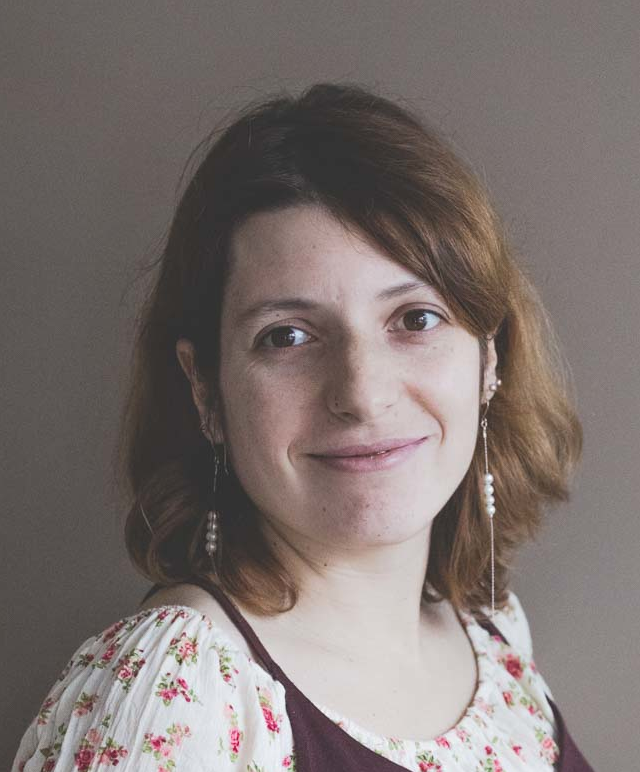
\includegraphics[scale=0.13]{Photo.png}
\end{minipage}

\vspace{0.5cm}

%----------------------------------------------------------------------------------------
%  EDUCATION
%----------------------------------------------------------------------------------------

\cvsect{Education}

{\large{Lomonosov Moscow State University,\\
Faculty of Geography,\\
Department of meteorology and climatology}}
\\\\

\begin{entrylist}
  \entry{2007 --- 2009}
  {Master's Degree,}
    {}
    {Thesis: ``Changes of cold season applied climatological characteristics in Russia in 1950--2006''}
  \entry{2003 --- 2007}
    {Bachelor's Degree}
    {}
    {\hyphenpenalty=10000 Thesis: ``Change of the intensity of snowfalls and its impact on expenses of cleaning main roads in Russian towns''}
\end{entrylist}

%----------------------------------------------------------------------------------------
%  EXPERIENCE
%----------------------------------------------------------------------------------------

\cvsect{Experience}

\begin{entrylist}
  \entry{2010 --- now*}
    {Junior researcher}
    {}
    {\
      Institute of Geography Russian Academy of Sciences, laboratory of climatology\\
      {\footnotesize* October 2017 moving to Germany, maternity leave with two children (were born in 2015 and 2019), part-time remote work in Institute of Geography RAS}
    }
  \entry{2009 --- 2015}
    {Lead expert}
    {}
    {\hyphenpenalty=10000 Aviamettelekom of Roshydromet (The Russian Federal Service for Hydrometeorology and Environmental Monitoring), department of marketing and development}
\end{entrylist}

%----------------------------------------------------------------------------------------
%  ADDITIONAL INFORMATION
%----------------------------------------------------------------------------------------

%\vspace{1.5cm}
\cvsect{Computer skills}\\
  Platforms: Windows, Linux\\
  Languages: SQL, Python\\
  Applications: MS Office and LibreOffice, Surfer, QGIS, ArcGIS\\\\
\cvsect{Additional information}
Participation in 13 international conferences, 7 field expeditions\\
12 articles in peer-reviewed journals\\
Languages: Russian --- native; English --- B1--B2; German --- A2-B1\\
Eligible to work in Germany (residence permit)

%----------------------------------------------------------------------------------------

\end{document}
